\documentclass[a4paper]{article}

\usepackage[utf8]{inputenc}
\usepackage{graphicx}

\parindent 0px

\title{Das Epische Theater}
\author{Alin Porcic}

\begin{document}

	\maketitle

	\newpage

	\section{Das Epische Theater}

        Das Epische Theater, ein von Bertolt Brecht geprägter Begriff, verbindet die zwei literarische Gattungen: die Dramatik und die Epik. In den 1920er Jahren experimentierten Bertolt Brecht und Erwin Piscator an einem spezeziellen  Drama. Sie versuchten die Darstellung von tragischen Einzelschicksalen auf der Bühne zu vermeiden und versuchten stattdessen gesellschaftliche Konflikte, wie zum Beispiel Kriege, Revolutionen oder soziale Ungerechtigkeit, durchschaubar aufführbar zu machen und den Zuschauer dazu bewegen, die Gesellschaft zum Positiven zu verändern. Nach Bertolt Brecht soll das Epische Theater durch die Demonstratation von gesellschaftlichen und politischen Widersprüchen den Zuschauer zu positiven Veränderungen in der realen Welt inspirieren.\\\\

        Der Zuschauer soll das Geschehen kritisch und emotionslos betrachten und sich dabei von den gezeigten Ereignissen distanzieren. Das Mitgefühl der Zuschauer zu den Figuren soll unterbunden werden und er soll während der Auffürhung gesellschaftliche Erkenntnisse sammeln können. Im Gegensatz zum aristoteleschen Theater hat das Epische Theater keinen Spannungbogen, jede Szene steht für sich und kann in der Reihenfolge verändert werden. Ein offener Schluss ist im Epischen Theater eher üblich.\\\\

	Die Verfremdungseffekte sind stilistische Methoden, die das Epische Theater anwendet, um die Entstehung von Spannung zu vermeiden. Bertolt Brecht ist der Meinung, dass die Spannung den Zuschauern im Denken und Lernen behindere und deshalb entfernt werden müsse. Das wird durch folgende Methoden erreicht:
        
        \begin{itemize}
	\item Der Szeneninhalt wird schon vor der Aufführung der jeweiligen Szenen erzählt. Damit weiß der Zuschauer was ihm erwartet und er kann sich ganz auf den Inhalt des Stücks konzentieren.
        \item Das Bühnenbild wird gezielt verändert, sodass der Zuschauer immer weiß, dass er sich im Theater befindet und die Ereignisse nicht real sind.
        \item Kommentare unterbrechen die Handlungen, Figuren treten aus ihren Rollen aus und wenden sich an das Publikum.
        \item Es wird zum Teil in Versen gesprochen.
        \item Die Schauspieler versuchen eine Distanz zur jeweiligen gespielten Figur aufzubauen, damit der Zuschauer den Protagonisten nicht als Identifikationsfigur wahrnehmen kann. Die Figuren können daher kritische betrachtet werden.
        \item Lieder werden eingebaut.
        \end{itemize}
        
        \newpage
        \section{Bertolt Brecht (1898 - 1956)}

	Bertolt Brecht wurde am 10.Febuar 1898 in Augsburg, Deutschland, geboren und wuchs in gesicherten ökonomischen und sozialen Verhältnissen auf. Sein Vater hatte keine höhere Schulausbildung, konnte sich aber in der Augsburger Haindl'schen Papierfabrik zum Direktor hoch arbeiten.\\\\
        Bertolt Brecht besuchte stadesgemäß das Realgymnasium und brachte regelmäßig gute, wenn nicht sehr gute Zeugnisse nach Hause.\\\\
        Schon im jungen Alter began Bertolt mit dem Dichten und arbeitet zusammen mit seinen Freunden an einer Schülerzeitung. Er verfasste Gedichte, Prosatexte und sogar ein einaktiges Drama, die Bibel. In den folgenden Jahren produzierte er weitere Gedichte und Dramenentwürfe.\\\\
        Nach dem Beginn des Ersten Weltkrieges 1914 gelang es ihm, eine Serie von Reportagen und Rezensionen in die lokalen und reginalen Medien unterzubringen (München-Augsburger Abendzeitung). 1916 verfasste er Gedichte, die in der späteren Sammlung 'Bertolt Brechts Hauspostille' eingebunden wurden. 1920 arbeitet er mit Erwin Piscator am Epischen Theater und verfasst weiter Dramen.\\\\

	\subsection{Werke}

        \begin{itemize}
        \item Baal
	\item Trommeln in der Nacht
	\item Mutter Courage und ihre Kinder
        \item Der gute Mensch von Sezuan
        \item Die Mutter
        \item Der Brotladen
        \item Die sieben Todsünden
        \item Die Maßnahme
        \item ...
          
        \end{itemize}
        
        \section{Mutter Courage und ihre Kinder}

	'Mutter Courage und ihre Kinder' ist ein Drama, welches von Bertolt Brecht im schwedischen Exil 1938/39 verfasst wurde und 1941 in Zürich uraufgeführt wurde. Im dramatischen Werk geht es um die Mutter Courage, die versucht mit dem Krieg Geschäfte zu machen und dabei alle drei Kinder verliert. Bertolt Brecht möchte mit diesem Werk Abscheu vor dem Krieg vermitteln und vor der kapitalistischen Gesellschaft.
        
	\subsection{Inhaltsangabe}        

	Anna Fierling, auch Mutter Courage genannt, zieht mit ihrem Marktwagen, ihren beiden Söhnen, dem mutigen Eilif, dem ehrlichen, aber dummen Schweizerkas und ihrer stummen Tochter Kattrin durch die Lande.\\
        In Südschweden wird Eilif von einem Feldwebel für den Krieg gewornem. Die sehr pessimistisch gestellte Mutter Courage sagt dem Feldwebel den Tod voraus, aber auch, dass ihre eigenen Kinder den Tod finden werden. Zwei Jahre später sieht sie ihren Sohn Eilif als Held in Polen wieder. Seine Heldentat, er hat einem Bauern das Vieh gestohlen, belohnt sie mit einer Ohrfeige. Gemeinsam mit einem finnischen Regimetn gerät Mutter Courage in Gefangenschaft der Katholiken. Als Schweizerkas die Regimentskasse in Sicherheit bringen will, wird er ertappt und vor dem Feldgericht verurteilt. Um ihn auslösen zu können, verpfändet Mutter Courage ihren Wagen, doch sie feilscht so lange, bis Schweizerkas erschossen wird. Als ihre Waren mutwillig zerstört werden, möchte sie sich beim Rittmeister beschweren, doch sie besinnt sich, denn es ist ihrer Meinung nach besser, im Krieg Handel zu betreiben, als Gerechtigkeit zu suchen. Ein protestantischer Feldprediger hilft ihr, sich dem katholischen Heer anzuschließen. Aufgrund eines ÜBerfalls auf Kattrin, wechselt Mutter Courage die Front. Eilif wird zum Tode verurteilt, weil er eine Bauersfrau umgebracht hat. Vier Jahre vergehen und Kattrin belauscht das Gespräch einiger kaiserlichen Soldaten, die die Stadt Halle strümen wollen und steigt auf das Dach des Hauses, um die Bewohner zu warnen. Es gelingt ihr auch, doch sie wird von einem Soldaten erschossen. Mutter Courage zieht mit ihrem Wagen alleine weiter. Sie hat alle drei Kinder verloren und nichts aus dem Krieg gelernt.
        
        \subsection{Interpretation}

        Im Exil 1938/1939 wird Brecht auf die dortige Literatur aufmerksam und stößt auf eine Erzählung von John Ludvig Runeberg (finnlandschwedischer Schriftsteller) in der eine mütterliche Marketenderin (=Händler, die die Truppen begleiten, verpflegen und medizinisch versorgen) vorkommt. Der Schauplatz und den Namen 'Courage' hat Brecht von Grimmelshausen ausgeliehen.\\
Die zentrale Frage des Stückes: Warum verteidigt eine Frau den Krieg, obwohl dieser ihre drei Kinder getötet hat? Um den Zuschauer immer wieder mit dieser Frage zu belästigen, werden im Stück auf die Mittel des Epischen Theaters gesetzt - der Zuschauer soll aus der passiven Beobachtungsrolle aussteigen und aktive am Stück teilnehmen. Dazu gehört zum Beispiel die kurze Inhaltsangabe vor jeder Szene, die Gesänge der Schauspieler, das unpassende Bühnenbild und so weiter.\\
Immer wieder werden unregelmäßig Lieder eingebaut, um auf den erzählten Inhalt zu deuten und zu interpretieren. Die Lieder werden nicht von der Mutter Courage gesungen, sondern von der Darstellerin. Dieser kleine Unterschied veranlasst das der Zuschauer den Darsteller nicht mit der Figur indentifizieren kann.\\
Alle Widersprüche laufen zu einer Figur zusammen: die Mutter Courage. Sie verteidigt den Krieg, obwohl dieser alle ihre Kinder genommen hat, da sie mit dem Krieg feilscht. Trotzdem ist die Mutter Courage davon überzeugt, dass sie nur das beste für ihre Kinder wolle. Nur wenige Male nimmt sie eine kritische Haltung ein, die aber nur von kurzer Dauer ist. Getrieben von der Gier und dem Überlebensdrang versucht sie überall mit ein bisschen Feilschen ein bisschen mehr Profit zu erwirtschaften.\\
Doch was lernt die Mutter Courage? Nichts - am Ende des Stücks steht sie am Anfang, nur ohne ihre Kinder.  

\section{Figurenkonstallation}
	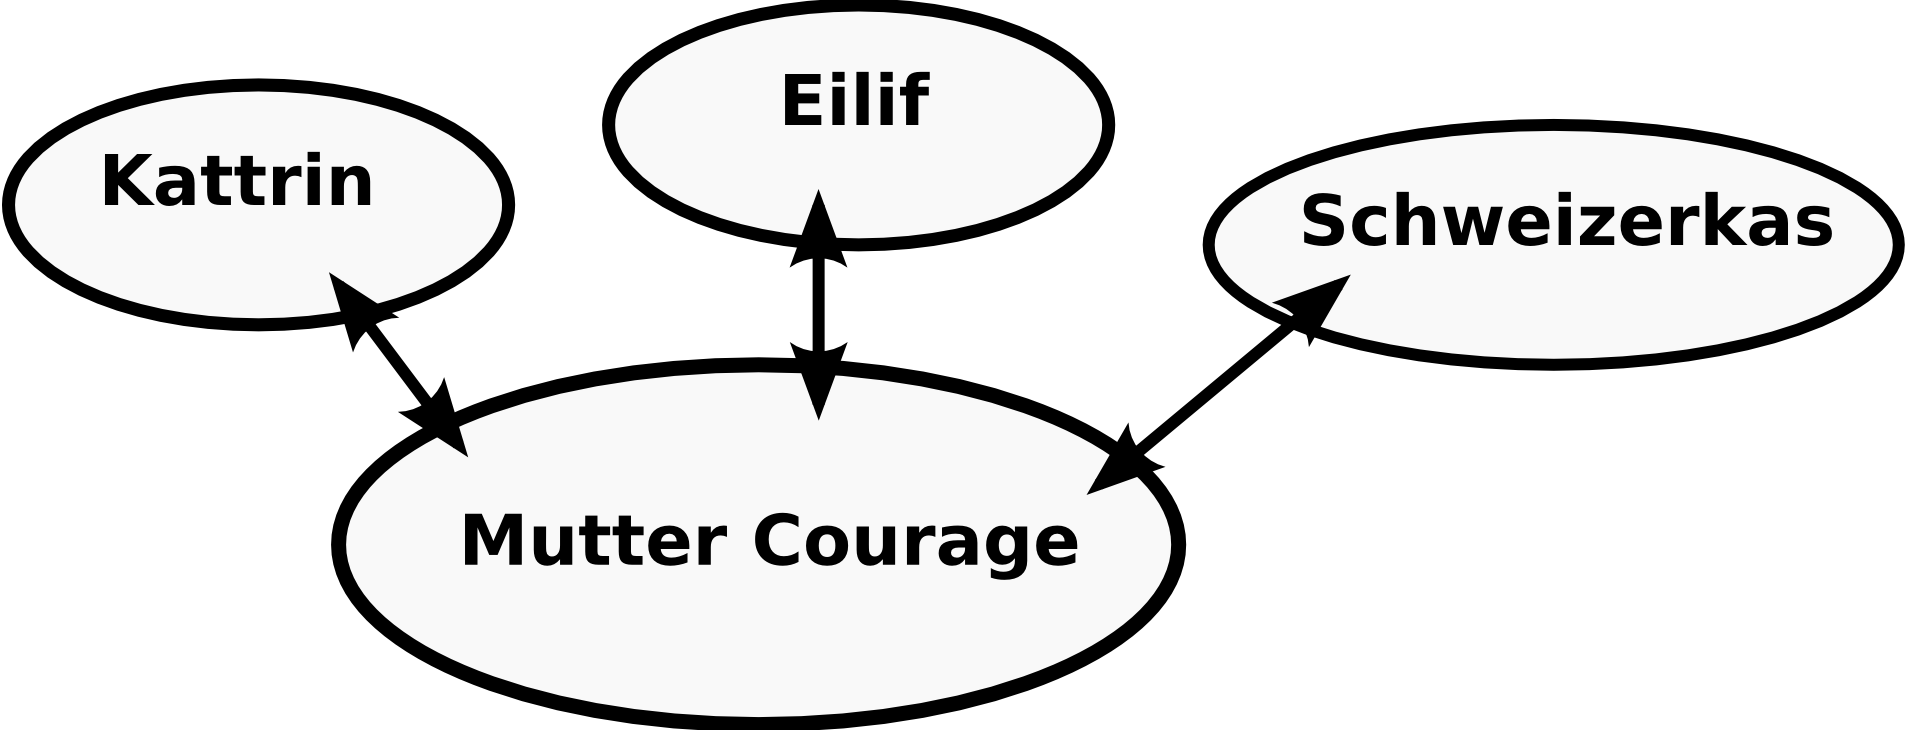
\includegraphics[width=250px]{img/figuren.png}
        
\end{document}
